\newpage
\section*{Appendix}

\section{Input features to density prediction module}
\label{app:input_features}

The authors use a density prediction module that is agnostic to the visual categories. Instead of feeding the features obtained from the feature extraction module directly, they rather use the correlation map between the exemplar features and image features as the input to the density prediction module. In Figure \ref{fig:orange_copmuted_features} we show an example of an input (correlation features) to the density prediction module.

\begin{figure}[htb]
	\centering
	\begin{tabular}{c}
		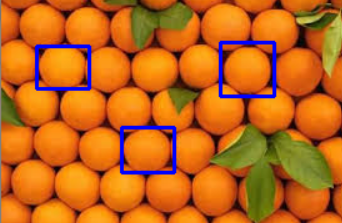
\includegraphics[width=0.15\linewidth]{fig/orange_bounding_boxes.png} \\ 
		(a) Input image with three exemplars \\
		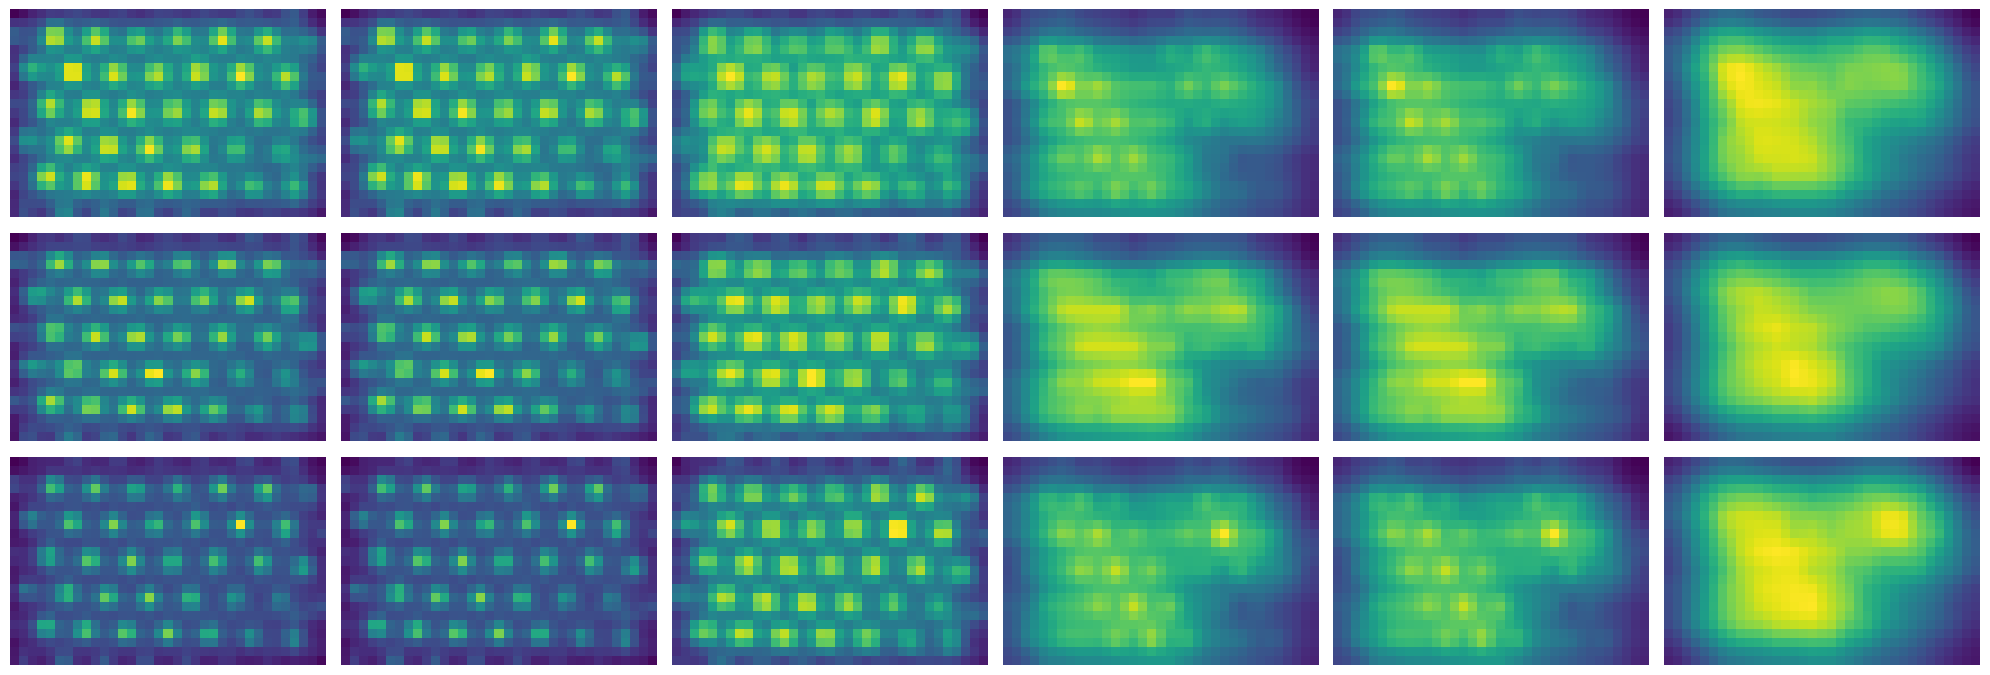
\includegraphics[width=0.8\linewidth]{fig/orange_features.png} \\
		(b) Correlation maps
	\end{tabular}
	\caption{Figure shows an example of an input image (a) from FSC-147 with three exemplars (blue rectangles), and correlation maps between exemplar and image features (b), that are fed to the density prediction module. Each row corresponds to one exemplar, while each column corresponds to one combination of scale (3 scales) and feature output from third or fourth block of ResNet-18.}
	\label{fig:orange_copmuted_features}
\end{figure}

\section{Images with the best and the worst relative MAE on test set without adaptation}
\label{app:no_adapt}

We visually inspect the images where absolute error normalized by the ground truth count is the highest or the lowest, and show some of the images in Figure \ref{fig:examples}. We can see that the algorithm predicts density maps with highest relative count error in cases where he predicts counts for wrong objects. In all three cases defined shapes which confuse the algorithm are present. Algorithm works the best on images, where the shape of the object it counts is well-defined and differs from the background, or there is no background at all. Adaptation in some cases improves the prediction, while in some cases it makes it worse. Thus, we investigate the affect of adaptation in the next section of appendix.

\begin{figure}[htb]
	\centering
	\begin{tabular}{cccc}
		\includegraphics[width=0.24\linewidth]{fig/7171_img.png} &
		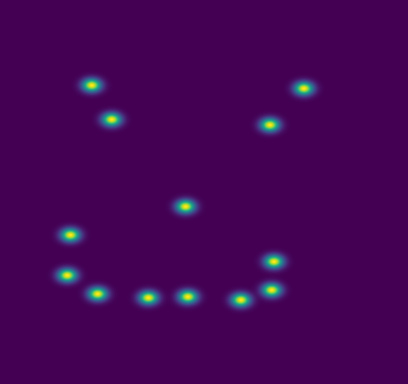
\includegraphics[width=0.24\linewidth]{fig/7171_gt.png} &
		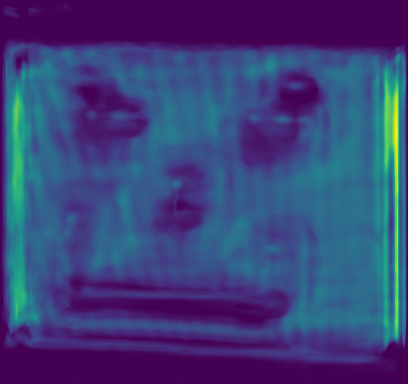
\includegraphics[width=0.24\linewidth]{fig/7171_pred.png} &
		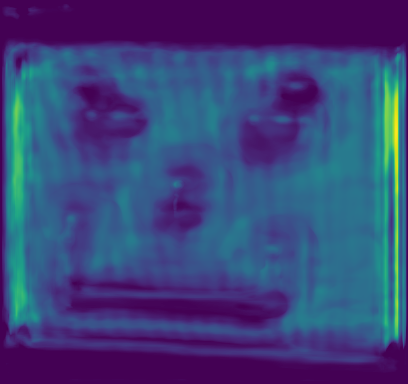
\includegraphics[width=0.24\linewidth]{fig/7171_pred_adapt.png} \\
		%7171.jpg & GT: 13 & Pred: 647.06 & Pred (A): 691.95 \\
		7171.jpg & GT: 13 & Pred: 647.7 & Pred (A): 670.5 \\
		\includegraphics[width=0.24\linewidth]{fig/5365_img.png} &
		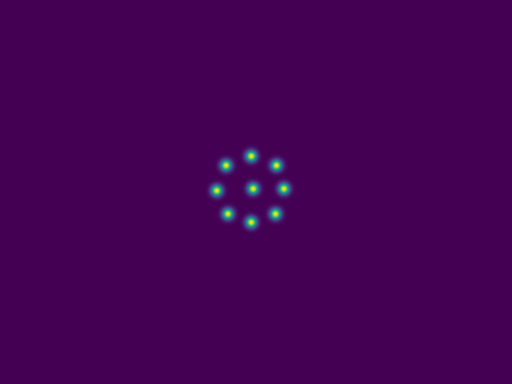
\includegraphics[width=0.24\linewidth]{fig/5365_gt.png} &
		\includegraphics[width=0.24\linewidth]{fig/5365_pred.png} &
		\includegraphics[width=0.24\linewidth]{fig/5365_pred_adapt.png} \\
		%5365.jpg & GT: 9 & Pred: 78.02 & Pred (A): 86.90 \\
		5365.jpg & GT: 9 & Pred: 75.7 & Pred (A): 73.7 \\
		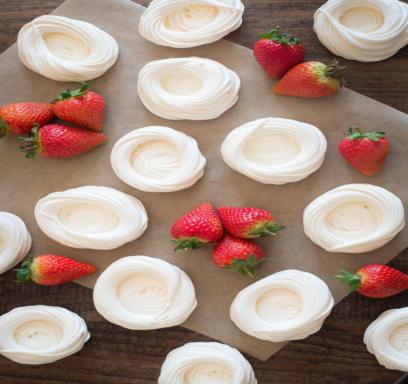
\includegraphics[width=0.24\linewidth]{fig/4885_img.png} &
		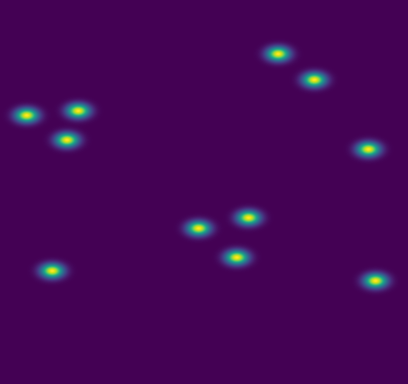
\includegraphics[width=0.24\linewidth]{fig/4885_gt.png} &
		\includegraphics[width=0.24\linewidth]{fig/4885_pred.png} &
		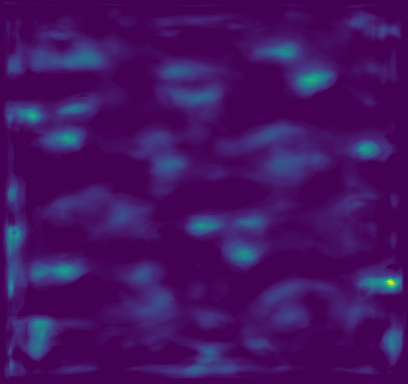
\includegraphics[width=0.24\linewidth]{fig/4885_pred_adapt.png} \\ 
		%4885.jpg & GT: 11 & Pred: 46.55 & Pred (A): 49.15 \\
		4885.jpg & GT: 11 & Pred: 35.0 & Pred (A): 45.2 \\
		\includegraphics[width=0.24\linewidth]{fig/2163_img.png} &
		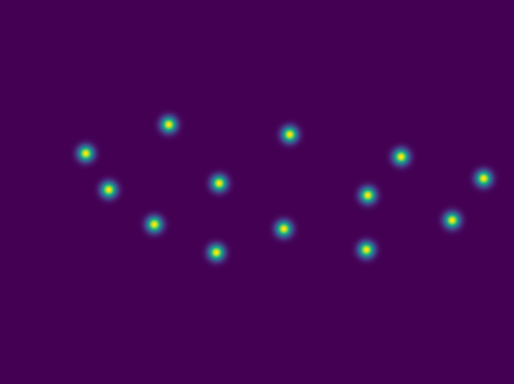
\includegraphics[width=0.24\linewidth]{fig/2163_gt.png} &
		\includegraphics[width=0.24\linewidth]{fig/2163_pred.png} &
		\includegraphics[width=0.24\linewidth]{fig/2163_pred_adapt.png} \\
		%2163.jpg & GT: 13 & Pred: 5.80 & Pred (A): 6.83 \\
		2163.jpg & GT: 13 & Pred: 5.9 & Pred (A): 6.4 \\
		\includegraphics[width=0.24\linewidth]{fig/4300_img.png} &
		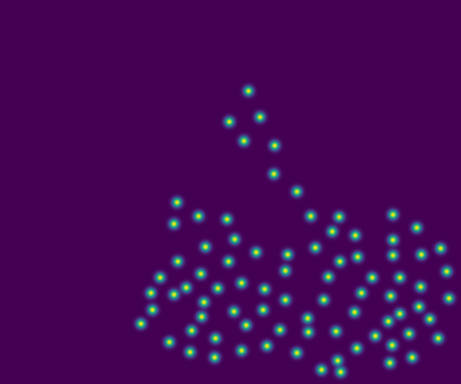
\includegraphics[width=0.24\linewidth]{fig/4300_gt.png} &
		\includegraphics[width=0.24\linewidth]{fig/4300_pred.png} &
		\includegraphics[width=0.24\linewidth]{fig/4300_pred_adapt.png} \\
		%4300.jpg & GT: 83 & Pred: 63.98 & Pred (A): 66.65 \\
		4300.jpg & GT: 83 & Pred: 63.7 & Pred (A): 63.0 \\
		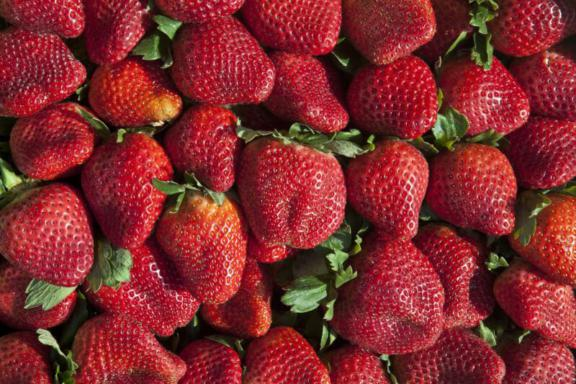
\includegraphics[width=0.24\linewidth]{fig/5811_img.png} &
		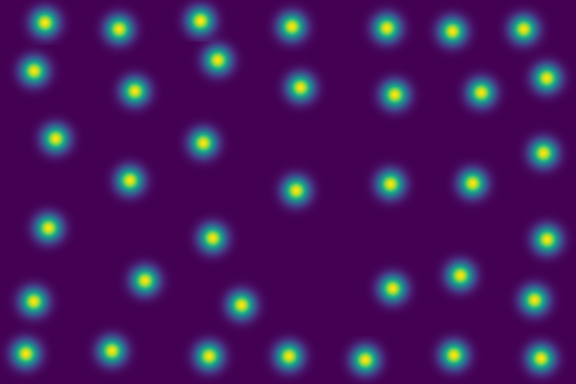
\includegraphics[width=0.24\linewidth]{fig/5811_gt.png} &
		\includegraphics[width=0.24\linewidth]{fig/5811_pred.png} &
		\includegraphics[width=0.24\linewidth]{fig/5811_pred_adapt.png} \\
		%5811.jpg & GT: 37 & Pred: 22.16 & Pred (A): 25.75 \\
		5811.jpg & GT: 37 & Pred: 22.1 & Pred (A): 24.7 \\
	\end{tabular}
	\caption{The first column represents input images, the second represents ground truth density maps, while the third and the fourth represent predicted density maps without and with test-time adaptation, respectively. The first three rows include cases where absolute error normalized by ground truth count is among the highest in the test set, while the last three rows where it is among the lowest.}
	\label{fig:examples}
\end{figure}

\section{Effect of adaptation on predictions}
\label{app:adapt}

We inspect on which images the absolute error normalized by the ground truth count is improved or worsened the most. We show examples of those images in Figure \ref{fig:adaptation_effect}. We do not observe any special pattern in the shown images. The main reason for a bigger impact of adaptation on those images is that their relative errors were quite high/low and consequently absolute changes in the prediction had a bigger impact on relative error.

\begin{figure}[htb]
	\centering
	\begin{tabular}{cccc}
		\includegraphics[width=0.24\linewidth]{fig/5365_img.png} &
		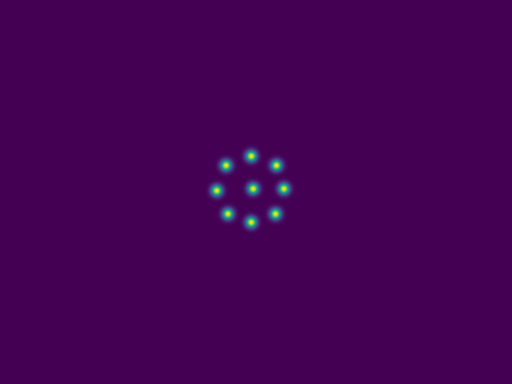
\includegraphics[width=0.24\linewidth]{fig/5365_gt.png} &
		\includegraphics[width=0.24\linewidth]{fig/5365_predict.png} &
		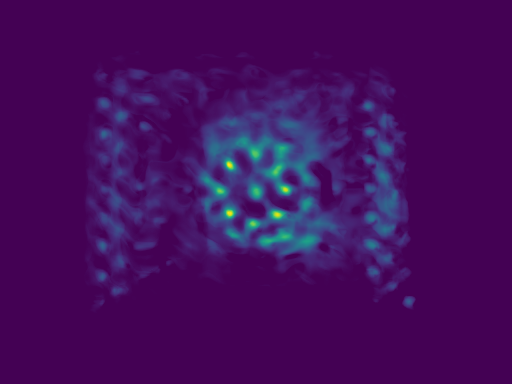
\includegraphics[width=0.24\linewidth]{fig/5365_adapt.png} \\
		5365.jpg & GT: 9 & Pred: 75.7 & Pred (A): 73.7 \\
		\includegraphics[width=0.24\linewidth]{fig/6266_img.jpg} &
		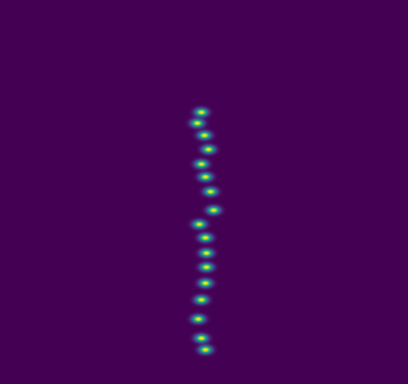
\includegraphics[width=0.24\linewidth]{fig/6266_gt.png} &
		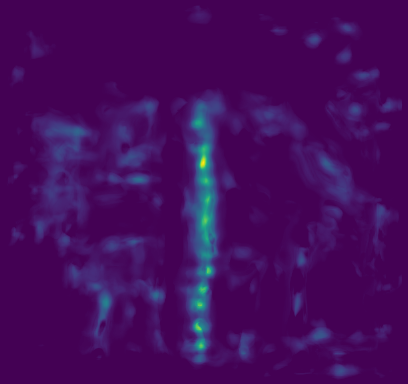
\includegraphics[width=0.24\linewidth]{fig/6266_predict.png} &
		\includegraphics[width=0.24\linewidth]{fig/6266_adapt.png} \\ 
		6266.jpg & GT: 17 & Pred: 65.6 & Pred (A): 62.6 \\ 
		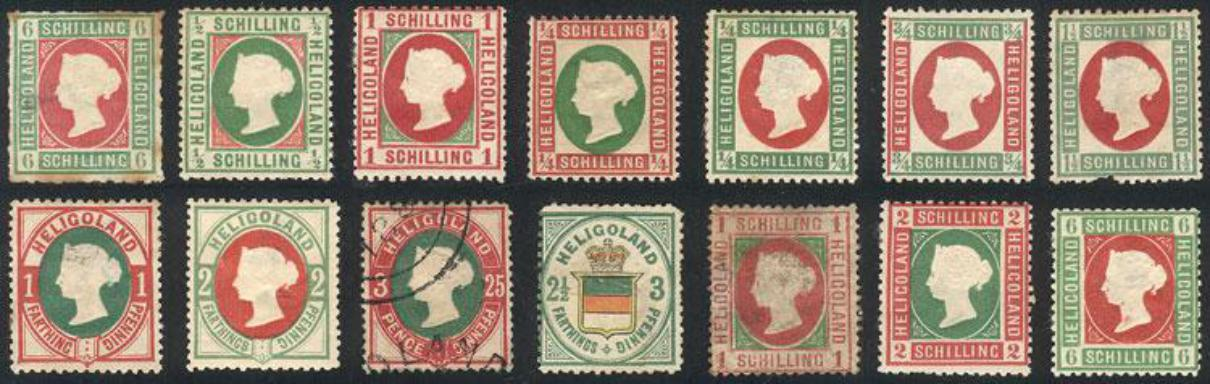
\includegraphics[width=0.24\linewidth]{fig/2910_img.jpg} &
		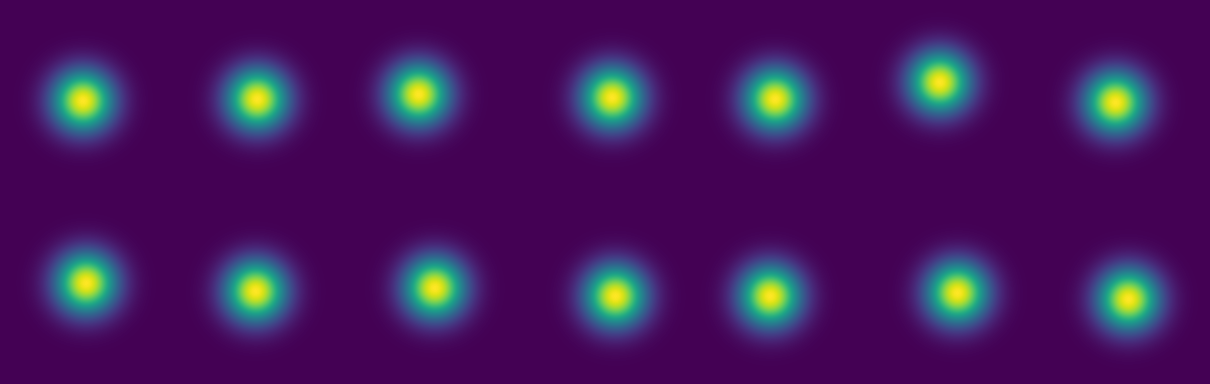
\includegraphics[width=0.24\linewidth]{fig/2910_gt.png} &
		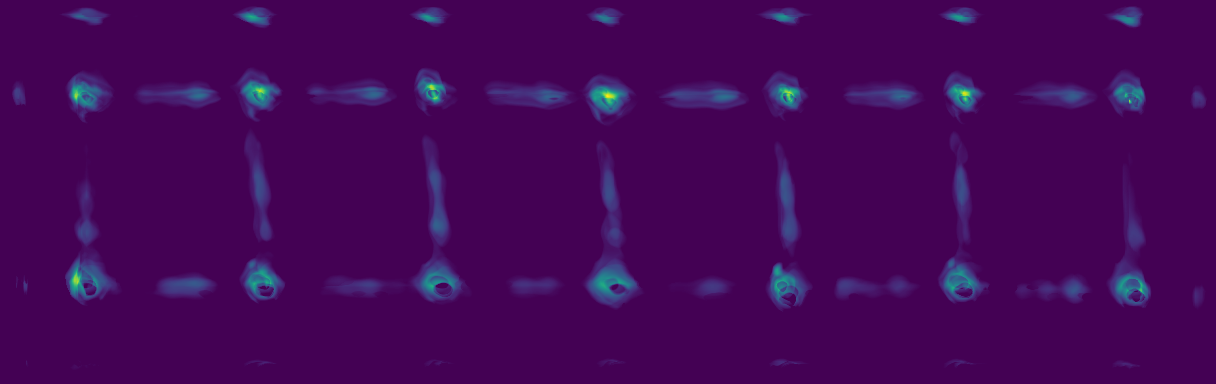
\includegraphics[width=0.24\linewidth]{fig/2910_predict.png} &
		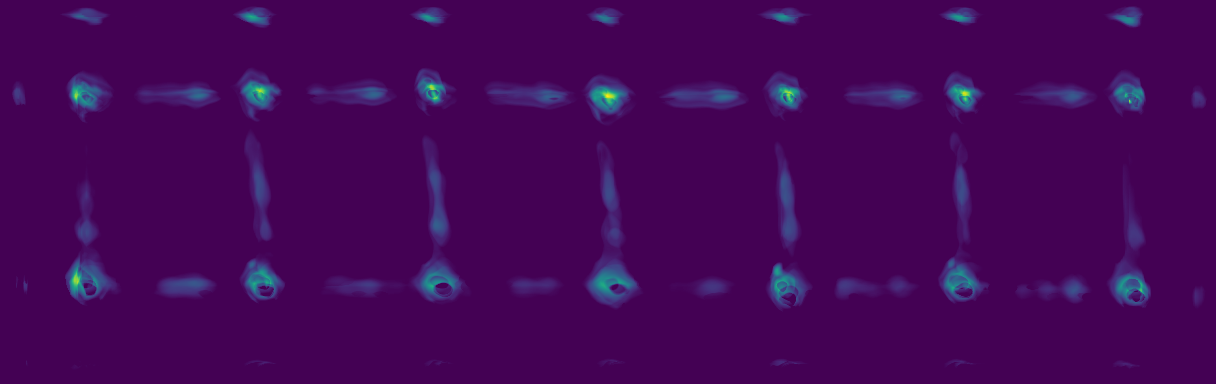
\includegraphics[width=0.24\linewidth]{fig/2910_adapt.png} \\
		2910.jpg & GT: 14 & Pred: 30.6 & Pred (A): 28.4 \\
		\includegraphics[width=0.24\linewidth]{fig/4112_img.jpg} &
		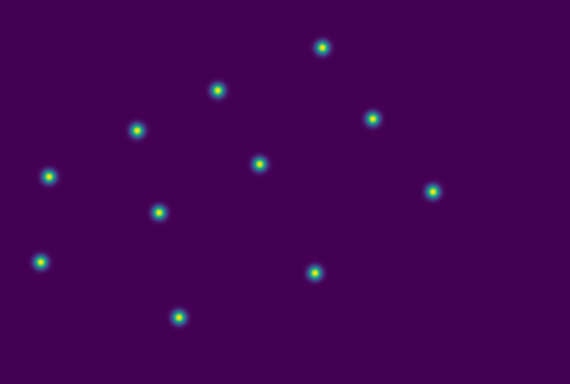
\includegraphics[width=0.24\linewidth]{fig/4112_gt.png} &
		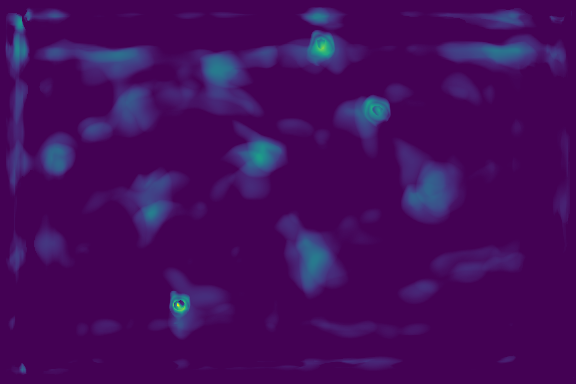
\includegraphics[width=0.24\linewidth]{fig/4112_predict.png} &
		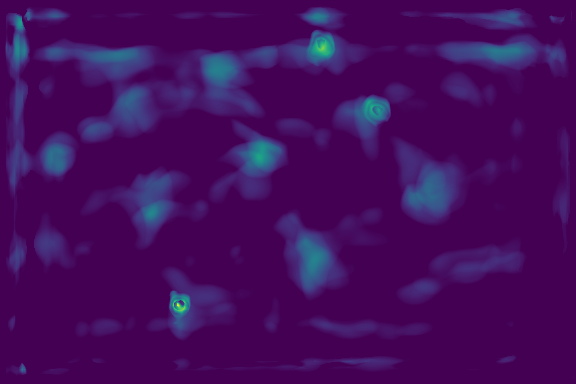
\includegraphics[width=0.24\linewidth]{fig/4112_adapt.png} \\
		4112.jpg & GT: 11 & Pred: 11.8 & Pred (A): 14.1 \\
		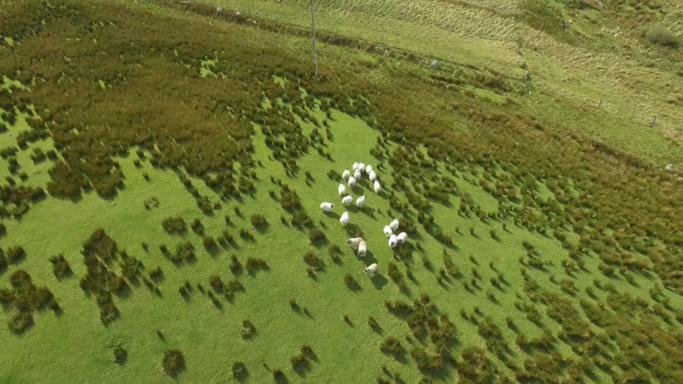
\includegraphics[width=0.24\linewidth]{fig/7639_img.jpg} &
		\includegraphics[width=0.24\linewidth]{fig/7639_gt.png} &
		\includegraphics[width=0.24\linewidth]{fig/7639_predict.png} &
		\includegraphics[width=0.24\linewidth]{fig/7639_adapt.png} \\
		7639.jpg & GT: 20 & Pred: 57.5 & Pred (A): 63.9 \\
		\includegraphics[width=0.24\linewidth]{fig/7171_img.png} &
		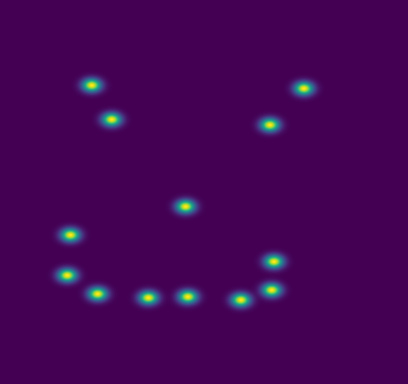
\includegraphics[width=0.24\linewidth]{fig/7171_gt.png} &
		\includegraphics[width=0.24\linewidth]{fig/7171_predict.png} &
		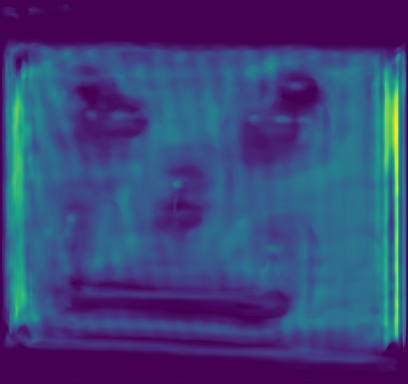
\includegraphics[width=0.24\linewidth]{fig/7171_adapt.png} \\
		7171.jpg & GT: 13 & Pred: 647.7 & Pred (A): 670.5 \\
	\end{tabular}
	\caption{The first column represents input images, the second represents ground truth density maps, while the third and the fourth represent predicted density maps without and with test-time adaptation, respectively. The first three rows include cases where the test time adaptation decreased relative error, while the last three rows include cases where the test time adaptation had a negative impact.}
	\label{fig:adaptation_effect}
\end{figure}
